\documentclass[12pt, a4paper]{article}
% пакеты
\usepackage{amsmath,amsfonts,amssymb,amsthm,mathtools}  
\usepackage{fontspec}         % пакет для подгрузки шрифтов
\setmainfont{Times New Roman}          % задаёт основной шрифт документа
\usepackage{leqno}
\usepackage{unicode-math}     % пакет для установки математического шрифта
\setmathfont{Asana Math}      % шрифт для математики

\usepackage{polyglossia}      % Пакет, который позволяет подгружать русские буквы
\setdefaultlanguage{russian}  % Основной язык документа
\setotherlanguage{english}
\usepackage{graphicx}
\graphicspath{}

\author{Маслова Инна}
\title{Домашнее задание 1}
\date{11.02.2017}
\begin{document}
\maketitle
\center{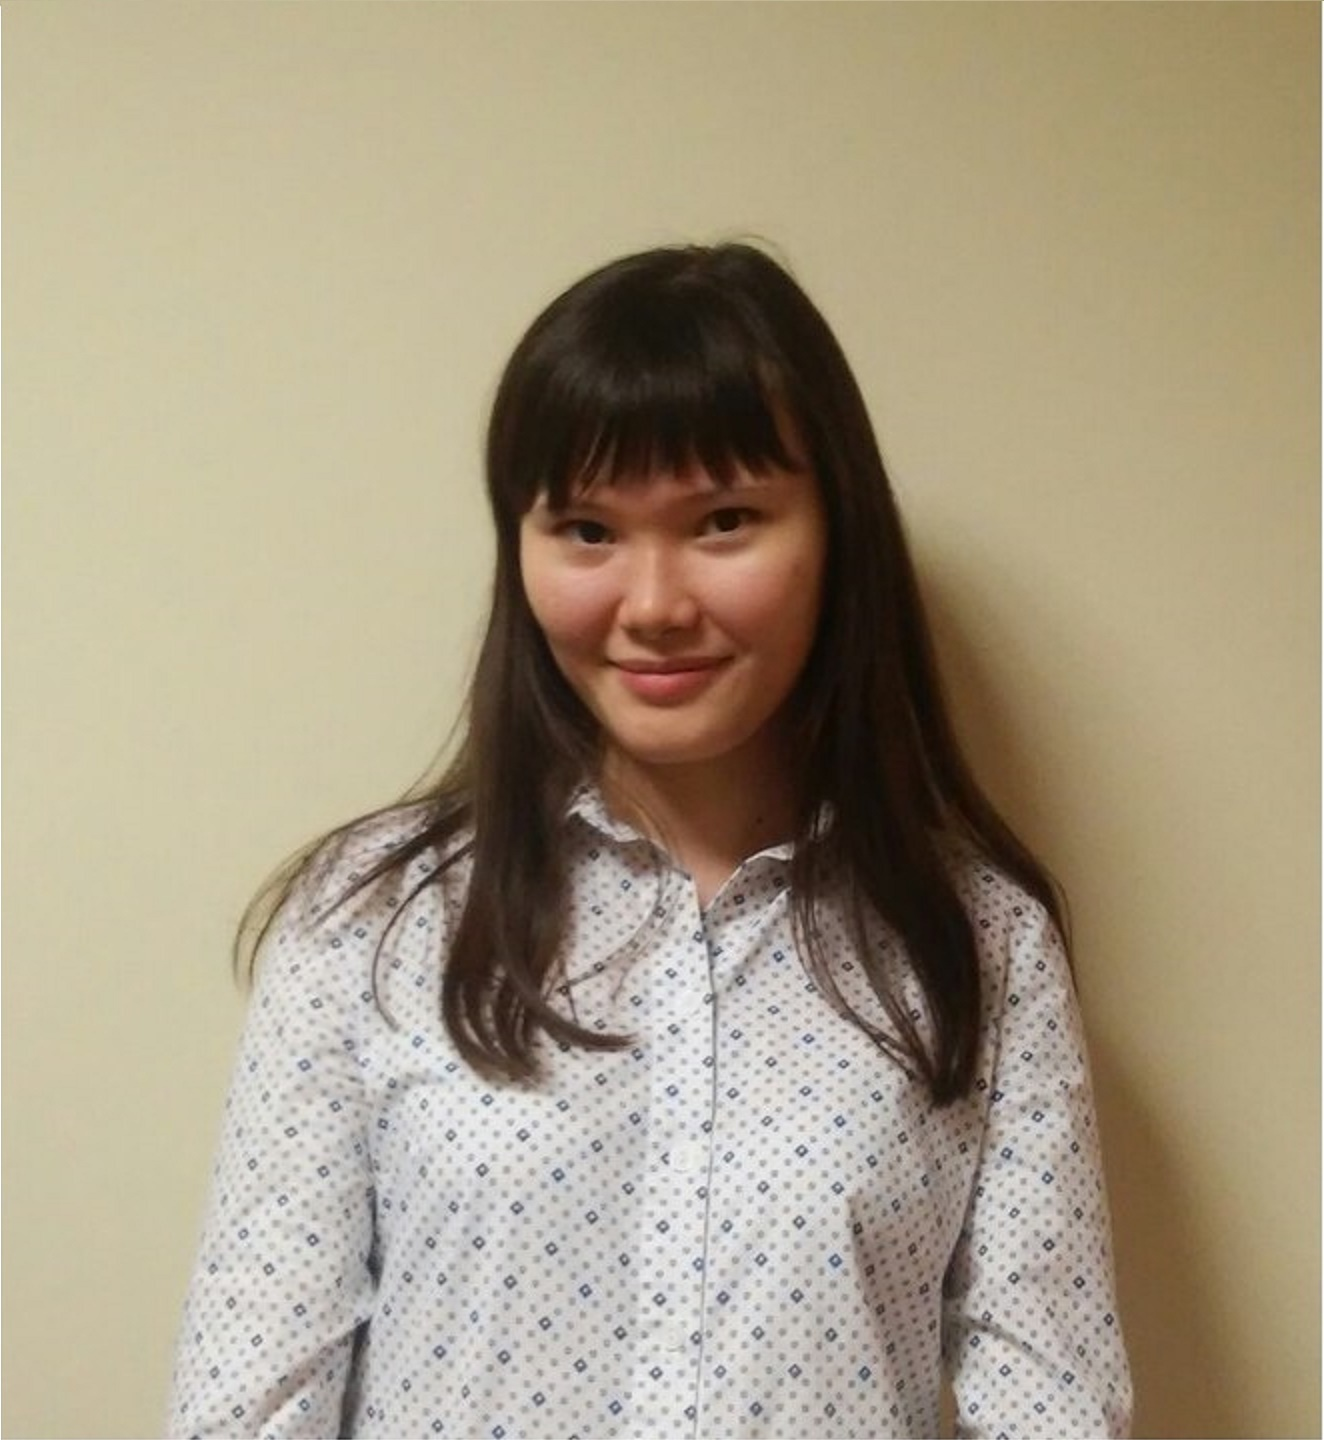
\includegraphics[scale=0.25]{photo}}
\section{10 фактов обо мне}
\begin{enumerate}
\item Я родилась в городе Элиста
\item Не особо люблю готовить, но иногда просыпается желание сделать какой-нибудь шедевр
\item Мне нравится чтение книг, описывающих события на протяжении всей жизни человека
\item Я живу в общаге
\item Побаиваюсь публичных выступлений
\item Я мало путешествовала, но надеюсь, что будущем изменить это
\item Когда не умираю от объема информации по учебе, пытаюсь найти что-то новое и интересное
\item Плохо разбираюсь в людях
\item Не умею плавать 
\item Временами меняю свои решения относительно того, как поступать в той или иной ситуации, что довольно сильно мешает жить
\end{enumerate}



\section{Формулы}
\begin{enumerate}
\item Полная запись леммы Ито \[ Y_t = Y_0+\int\limits_0^t f_w'(W_u,u)\,dW_u+\int\limits_0^t f_t'(W_u,u)\,du+\frac{1}{2} \int\limits_0^t f_{WW}''(W_u,u)\,du \tag{æ}\label{1} \] 
\item Оценки коэффициентов для множественной регрессии
\def \b{\hat{\beta}}
 \def \B { 
 \begin{pmatrix}
 \b_1 \\ \b_2 \\ \vdots \\ \b_n
 \end{pmatrix}}
 
 \def \x {
 \begin{pmatrix}
  x_{1,1} & x_{1,2} & \cdots & x_{1,k} \\
  x_{2,1} & x_{2,2} & \cdots & x_{2,k} \\
  \vdots  & \vdots  & \ddots & \vdots  \\
  x_{n,1} & x_{n,2} & \cdots & x_{n,k}
 \end{pmatrix}}

\def \X'{ 
 \begin{pmatrix}
  x_{1,1} & x_{2,1} & \cdots & x_{k,1} \\
  x_{1,2} & x_{2,2} & \cdots & x_{k,2} \\
  \vdots  & \vdots  & \ddots & \vdots  \\
  x_{1,n} & x_{2,n} & \cdots & x_{k,n}
 \end{pmatrix}}
 
\def \Y {  
 \begin{pmatrix}
 Y_1 \\ Y_2 \\ \vdots \\ Y_n
 \end{pmatrix}}
 \begin{align*}
  \B= \left(\X'* \x \right)^{-1} * \\
  \X'* \Y \tag{ææ}\label{2} 
\end{align*}

\item Бином Ньютона 
\begin{multline*}
(a+b)^n = \sum_{k=0}^{n} C^k_n b^k a^{n-k}=\\
=a^n+na^{n-1}b+\frac{n(n-1)}{1 \cdot 2}a^{n-2}b^2+\ldots+\\
+\frac{n \cdot (n-1)\cdot \ldots \cdot(n+k+1)}{1 \cdot 2 \cdot \ldots \cdot k}a^{n-k}b^k+ \ldots+b^n \tag{æææ}\label{3} 
\end{multline*}
\item Первый замечательный предел \[\lim_{x \to 0} \frac{\sin x}{x} = 1 \tag{ææææ}\label{4} \]

\item Разложение в ряд Тейлора
\[ \sin x = x - \frac{x^3}{3!}+\frac{x^5}{5!}-\frac{x^7}{7!}+ \cdots +(-1)^{m-1}\frac{x^{2m-1}}{(2m-1)!}+ \cdots \tag{æææææ}\label{5}
\] 
\item "Длинный логарифм" \[ \int \frac{dx}{\sqrt{x^2 \pm a^2}}= \ln|x+\sqrt{x^2 \pm a^2}|+C \tag{ææææææ}\label{6}
\]
\end{enumerate}


\begin{enumerate}
\item Мне нравится \eqref{1} больше всех, потому что, несмотря на длинную запись, она проста в запоминании и у нее есть замечательный краткий вариант, по которому можно составить полную формулу.
\item Формула \eqref{2} мне нравится, потому что она позволяет вычислить оценки коэффициентов для множественной регрессии в отличие от системы уравнений.
\item Формула \eqref{3} безумно полезная, так как позволяет разложить сумму двух слагаемых в $2,3,4$ и т.д. степенях
\item \eqref{4} красивая формула с красивым названием.
\item Я считаю \eqref{5} очень гармоничной формулой, которую так же нетрудно запомнить
\item \eqref{6} я не особо люблю, так как на $1$ курсе мучалась с запоминанием этой формулы. 
\end{enumerate}
\end{document}